\label{Chapter1}

\section{Μέρος πρώτο: εκμάθηση μιας νέας σημειακής λειτουργίας}

\subsection{Υλοποίηση της σύναρτησης solarize}

To \textbf{solarize} είναι μία σύναρτηση στην επεξεργασία είκονας η οποία επιτρέπει δημιουργεί το \textbf{φαινόμενο Sabattier}.
Το φαινόμενο Sabattier είναι το φαίνομενο στις φωτογραφίες, όπου η εικόνα είναι μαγνητοσκοπημένη σε ένα αρνητικό.

\begin{problem}
	Θα πρέπει να δημιουργηθεί μία συνάρτηση, η οποία θα υλοποιεί το φαινόμενο Sabattier και στην συνέχεια θα την κάνει ασπρόμαυρη.
\end{problem}

Αυτό μπορεί να υλοποιηθεί πολύ εύκολα με την χρήση του NumPy.
Το numpy κοιτάει τις τιμές της εικόνας και όπου είναι μεγαλύτερο από την τιμή κατωφλίου (threshold), τότε βάζει την αντιθέτη τίμη, διαφορετικά δεν την αλλαζεί.

\begin{lstlisting}[language=Python, caption=Solarize Function]
def solarize(image, threshold):
    return np.where((image < threshold), image, ~image)
\end{lstlisting}

\subsection{Εφαρμογή της συνάρτησης Solarize}

\begin{figure}[th]
	\centering
	
\includegraphics[width=100mm]{Figures/zelda}
	\caption[The Legend of Zelda - The Windwaker HD]{Screenshot από το βιντεοπαιχνίδι <<The Legend of Zelda - The Windwaker HD>> της Nintendo, 2013}
	\label{fig:zelda}
\end{figure}

Η συνάρτηση θα χρησιμοποιήσει στην είκονα του σχήματος~\ref{fig:zelda}. Οι τιμές του threshold πρόκειτε να είναι 64, 128 και 192.

\begin{figure}[th]
	\centering
	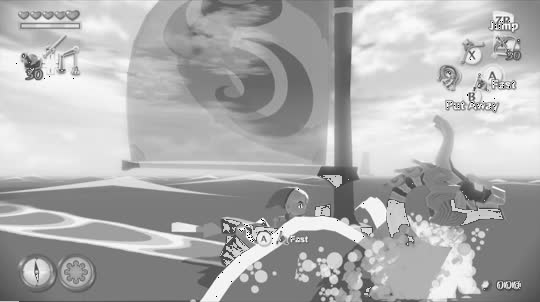
\includegraphics[width=100mm]{Figures/threshold_64}
	\caption[The Legend of Zelda - Windwaker HD Solarized 64 Threshold]{Solarized με τιμή του Threshold 64}
	\label{fig:threshold_64}
\end{figure}

\newpage
\subsection{Αποτελέσματα εφαρμόγης}

Τα αποτελέσματα των διαφορετικών τιμών του threshold εμφανίζονται στα σχήματα~\ref{fig:threshold_64},~\ref{fig:threshold_128} και~\ref{fig:threshold_192}.
Παρατηρώντας τα αποτελέσματα, μπορεί να παρατηρηθεί ότι τόσο πιο πολύ μεγαλώνει η τιμή του threshold, τόσο πιο πολύ η original εικόνα δεν είναι αναγνωρίσιμη.

\begin{figure}[th]
	\centering
	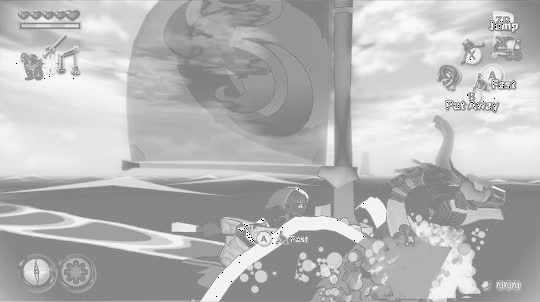
\includegraphics[width=100mm]{Figures/threshold_128}
	\caption[The Legend of Zelda - Windwaker HD Solarized 128 Threshold]{Solarized με τιμή του Threshold 128}
	\label{fig:threshold_128}
\end{figure}

\begin{figure}[th]
	\centering
	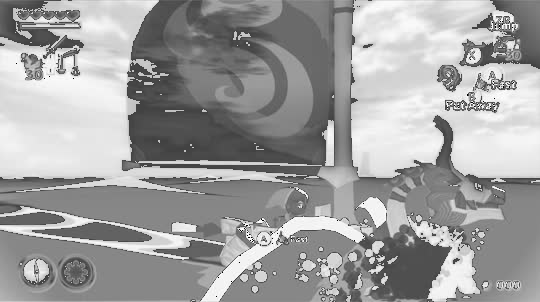
\includegraphics[width=100mm]{Figures/threshold_192}
	\caption[The Legend of Zelda - Windwaker HD Solarized 192 Threshold]{Solarized με τιμή του Threshold 192}
	\label{fig:threshold_192}
\end{figure}
